\documentclass{puzz}
\usepackage{wrapfig}

\begin{document}

\puzztitle{Puzzle 2: Clock Tower}

\begin{wrapfigure}{r}{0.15\textwidth}
    \centering
    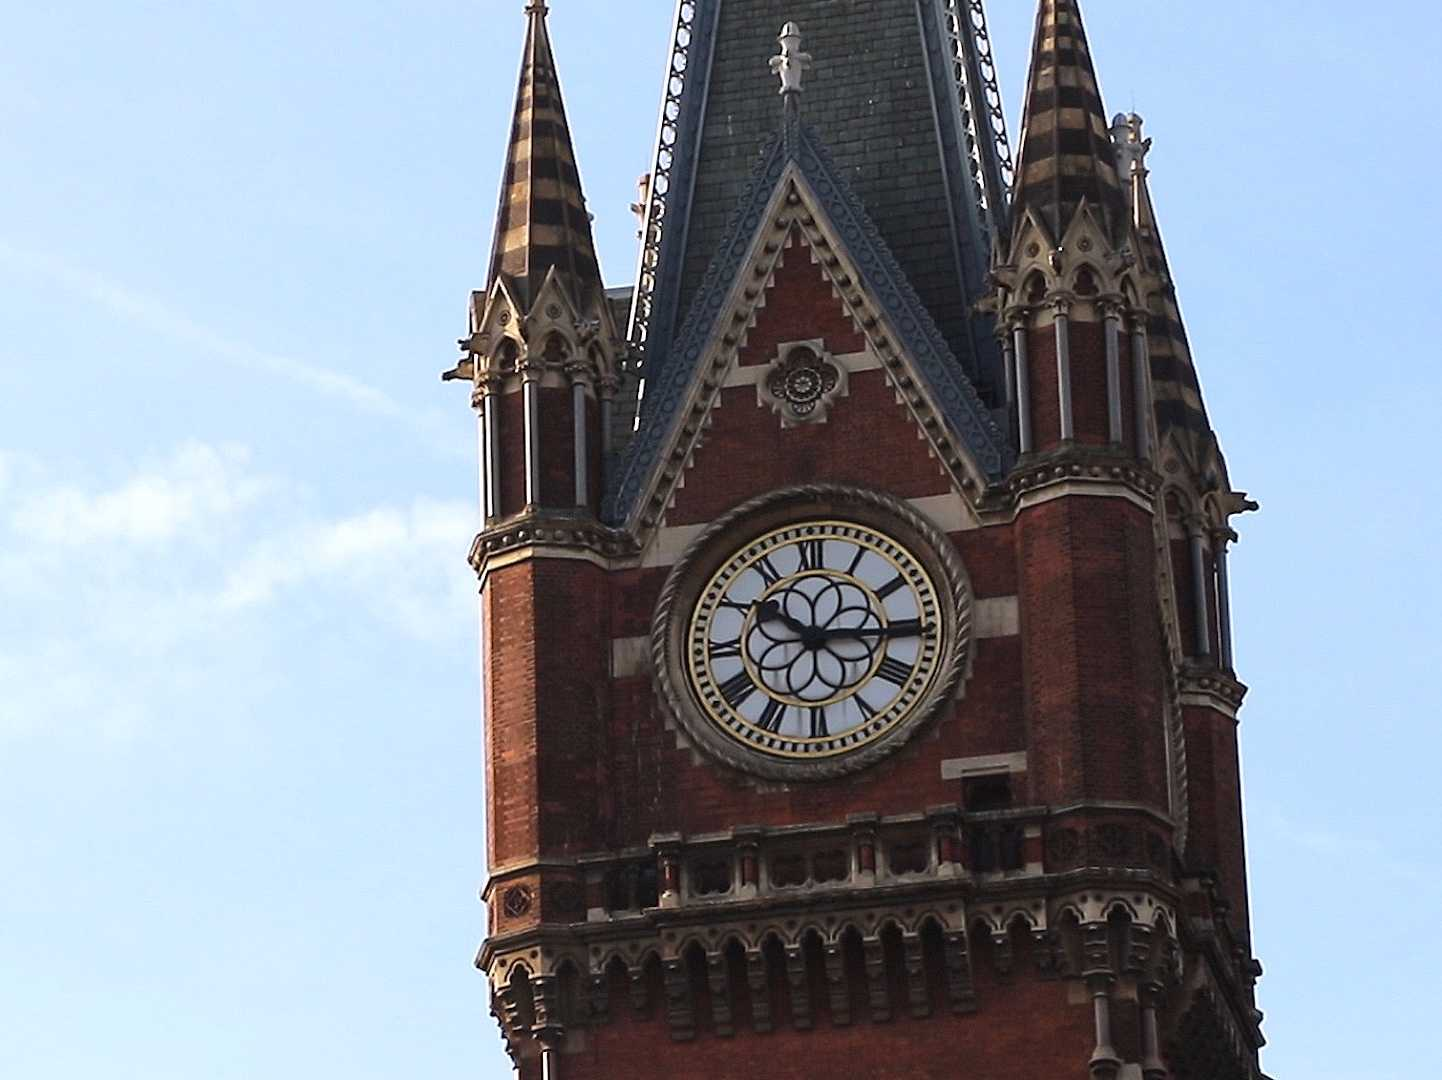
\includegraphics[width=0.15\textwidth]{graphics/clocktower}
\end{wrapfigure}

Your job is to clean a clock at the top of a 50-meter tall clock tower. The
tower has an elevator you can take to the cleaning platform at the top.

The elevator has been malfunctioning: normally you would just press \emph{up}
or \emph{down} to go all the way to the top or the bottom, but now it moves a
variable number of meters up or down with each press. Through a complex series
of button pushing, you've figured out this is the pattern:

\begin{center}
    \ttfamily
    7 2 11 18 5 10 9 8 5 3 2 2 3 5 10 4 5 1 3 10 4 2 1 5 16 8 16 18 10 6
\end{center}

For example, if you press \emph{up} initially, you will move up 7 meters. At
this point, you can either press \emph{down} or \emph{up}, moving you to
either 5 or 9 meters on the tower, respectively.

If the elevator rises above 50 meters, it will fall off its mechanism and you
will fall to your death. If the elevator is instructed to move below the 0
meter mark, it will break permanently. For example, from 9 meters, you cannot
move down 11 meters or the elevator will break.

Give a sequence of moves written as a string of the letters \texttt{U} and
\texttt{D} (corresponding to up and down, respectively) which will:

\begin{enumerate}
    \item Bring you to exactly 50 meters up the tower so you can perform the
        cleaning.
    \item Bring you to exactly the 0 meter mark so you can get down once the
        clock has been cleaned.
    \item Does not cause you to fall to your death or break the elevator, that
        way you can repeat the same sequence of moves in the future to clean it
        again.
\end{enumerate}

You do not have to use all of the moves in the pattern, as the pattern seems to
reset for the next time you have to clean. You cannot make more than 30 moves,
as the elevator will stop and you will be stuck.

Note: there are many correct answers to this puzzle. You only have to provide
one.
\end{document}
